\documentclass[12pt, preprint]{aastex}
\usepackage{hyperref}
\usepackage{color}
\newcommand{\niceurl}[1]{\href{#1}{\textsl{#1}}}

\begin{document}

\title{A Field Guide to the Word ``Optimal'' in Astronomy}

\author{%
Dustin Lang\altaffilmark{1,2}%
}
\altaffiltext{1}{%
  Dunlap Institute and Department of Astronomy \& Astrophysics,
  University of Toronto,
  50 Saint George Street, Toronto, ON, M5S 3H4, Canada
}
\altaffiltext{2}{%
  Department of Physics \& Astronomy,
  University of Waterloo,
  200 University Avenue West, Waterloo, ON, N2L 3G1, Canada
}
\date{\centering April 1, 2016}

\begin{abstract}
The word ``optimal'' is used widely in astronomy, but its semantics
in the astronomical literature
may be unfamiliar to researchers from other fields.  Here we give
our interpretations of various ways the word is used in the literature.
\end{abstract}

\keywords{%
April 1; Optimality; Astronomy literature}

\section{Introduction}

Use of the word ``optimal'' in the abstracts of papers posted to the
arXiv pre-print service has been increasing for the last 15 years, as
shown in Figure 1.  We used the arXiv API to query articles in the
``astro-ph'' category containing the term ``optimal'' in the abstract.
A total of 3159 articles with publication dates earlier than 2016
April 1 were returned.  With a total number of articles around
182,000, roughly $1.7\%$ of all astro-ph articles contain the word
``optimal''.  The total number of articles per year was compiled from
the summary statistics pages on the arXiv web site.\footnote{The
  query, data files, and the script used to generate the figures are
  included alongside the source of this paper, at
  \niceurl{https://github.com/dstndstn/shmoptimal}.}  Since use of the
word ``optimal'' in the astronomical literature continues to grow, and
since interdisciplinary research has become more popular, it becomes
more important for astronomers and researchers from other fields to
share not only vocabulary but also semantics.

\begin{figure}[ht!]
  \begin{center}
    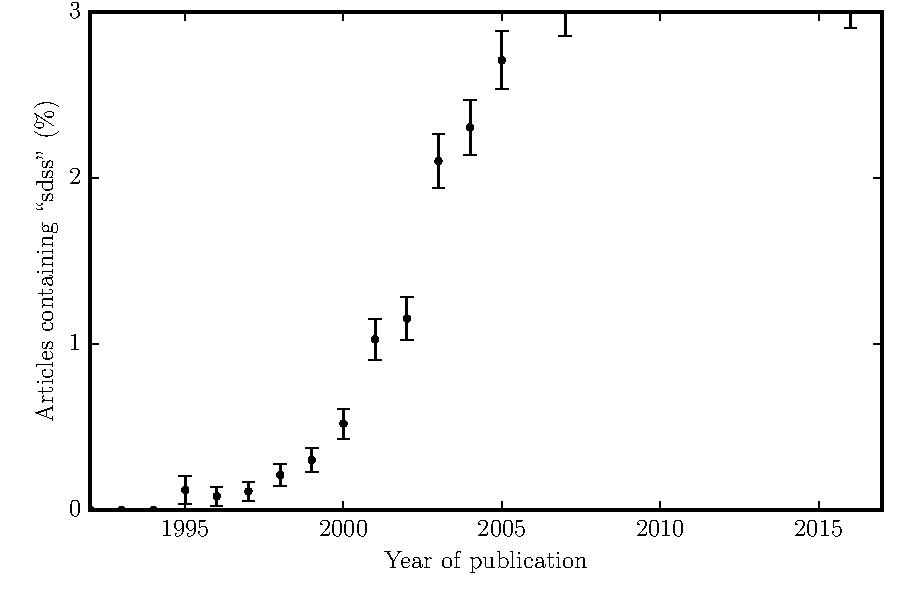
\includegraphics[width=0.8\textwidth]{yearly.pdf}
  \end{center}
  \caption{Growth of the word ``optimal'' in the abstracts of arXiv
    astro-ph preprints.  The error bars are based simply on the square
    root of the number of appearances of the word ``optimal'' per
    year, that is, assuming Poisson statistics.  Notice that the error
    bar for 2016 is larger because we only have data before April 1.}
\end{figure}


Before exploring the use of the word in the astronomical literature, let
us present definitions that might be recognizable to researchers from other
disciplines.

\begin{description}
\item[Optimal (of a parameter):] achieving the maximum of a
  well-specified scalar objective function.  That is, a parameter
  $\hat{\theta}$ can be said to be \emph{optimal} with respect to $f$
  if and only if
  \[
  \hat{\theta} = \arg\max_{\theta} f(\theta)
  \]
\item[Optimal (of a method, algorithm, or procedure):] achieving the
  best possible value of a specified scalar performance metric among a
  specified group of algorithms.
  %
  % For example,  ... Cramer--Rao
  %
\end{description}

\section{``Optimal'' in Astronomy}

A variety of uses of the word ``optimal'' can be found in the 
astronomical literature.
Here we show a number of examples with our interpretations of their
semantics.
%
Specific references to the literature have been suppressed, but in the
name of fairness, these examples are paraphrased from documents
coauthored by the authors of this guide.

\paragraph{``We present an optimal algorithm.''}
The authors present a good algorithm.  And by good, they
mean that they like it.  They like it because they wrote it, and it
even seemed to work better on the \emph{two} different test images
they ran it on.  At least, it looked better to them.  They plan
to make the code public in the near future.

\paragraph{``\emph{A} is more optimal than \emph{B}.''}
Neither \emph{A} nor \emph{B} is any good.  The phrase ``more
optimal'' of course indicates that the writer has never climbed to the
top of a hill and has not in any way quantitatively evaluated \emph{A}
versus \emph{B}.  Interestingly, this also hints that \emph{B} has not
been shown to be optimal, because if it had been, it would be
obviously fruitless to search for a superior \emph{A}.

\paragraph{``It is not clear that this method is optimal.''}
The method is horrible, but it was written by the author's supervisor
so the author is afraid to criticize it.

\paragraph{``Data set \emph{A} is nearly optimal for our science.''}
The authors have access to data set \emph{A}.

\paragraph{``Further simulation is required to optimize the survey design.''}
The authors have no idea what they are going to do.

\paragraph{``This is an ``optimal'' method.''}
Even the authors know the method is not optimal, but they just can't bring
themselves to write ``good'' instead.

\paragraph{``We chose optimal parameters $\alpha=1000$ and $\beta=7.42$
  for our production run''} The authors chose the number $1000$ because
it is a round number and the parameter $\alpha$ doesn't seem to do
anything at all, and $7.42$ because any other value of $\beta$ they
try causes the code to segfault.

\paragraph{``Our strategy optimally maximizes \emph{A} and \emph{B} while minimizing \emph{C}.''}
The survey strategy code was written in Perl by a grad student who
graduated a decade ago and now works for an insurance company.  Nobody
else in the lab can even read the code, never mind modify it, and it
uses parameters for a different telescope than the one the survey will
be carried out on.  Due to an elaborate series of bugs, it achieves
median performance on \emph{A} and random performance on \emph{B},
while maximizing \emph{C}.

\paragraph{``This method could be further optimized.''}
The authors have not optimized it yet and have no plans to do so.

% \paragraph{``We set the parameter to optimally trade off between \emph{A} and \emph{B}''}
% The authors set the parameter to halfway between what is best for
% \emph{A} and what is best for \emph{B}.

\paragraph{``Our pilot survey aimed at an optimal selection of targets''}
The authors tried really hard.

\paragraph{``As shown in Lemma 4, the variance of our estimator saturates
the Cram\'er--Rao bound''}
This was written by the authors' collaborator from the Statistics Department
and they are afraid to ask what it means.


\section{Conclusions}

We hope that this guide will optimize communication between astronomers
and collaborators from other disciplines.

\end{document}
